\documentclass[11pt]{article}
\usepackage[a4paper,margin=24mm]{geometry}
\usepackage{amsmath,amssymb,booktabs,graphicx,siunitx,enumitem,xcolor,hyperref}
\usepackage{microtype}
\graphicspath{{figures_v2/}}
\hypersetup{colorlinks=true,linkcolor=blue,citecolor=blue,urlcolor=blue}
\sisetup{round-mode=places,round-precision=3,detect-all}
\title{Network-feasible recovery scheduling for repeated distribution-flexibility services: an AC--SOC benchmark on the IEEE 13-node feeder}
\author{Siqiang Zhao$^{1,*}$ \and Fengxiang Zhang$^{1}$}
\date{}

\newcommand{\kw}[1]{#1~kW}
\newcommand{\pct}[1]{\SI{#1}{\percent}}

\begin{document}
\maketitle

\noindent\textsuperscript{1}[Department, institution, city, country to be completed].\\
\textsuperscript{*}Corresponding author: [name and e-mail to be completed].

\begin{abstract}
Repeated distribution-flexibility services couple battery state of charge (SOC) with time-varying feeder headroom. We formulate a two-call contract with constant service power, two two-hour service windows, declared recovery windows, and an exact terminal SOC. An isolated OpenDSS snapshot supplies AC-tested charging and export bounds for each half-hour profile, and an offline full-horizon linear program schedules recovery using the complete realized trajectory. The benchmark is compared with fixed recovery, a short-horizon myopic rule, and a copper-plate energy-only counterfactual. Using public Ausgrid profiles, a strict fixed-denominator mask retained 219 of 365 calendar dates and 2,188 baseline-AC-feasible date--group units at each of two IEEE 13-node single-phase placements. The date-cluster estimate of feasible service power was \kw{128.526} (95\% CI 125.981--131.154) at 611.3 and \kw{138.511} (134.811--142.131) at 634.1 for the full-horizon benchmark. Its paired difference from the myopic rule was 0.000 kW at 611.3 and \kw{2.433} (1.682--3.293) at 634.1. The energy-only schedules failed AC replay for every baseline-feasible unit, whereas the full-horizon benchmark replayed successfully for all such units. The results show that the value of anticipatory recovery is location dependent and that an energy-only offer can be materially optimistic. The benchmark is an offline screening workflow; it does not provide an online policy, a market valuation, or a probabilistic delivery guarantee.
\end{abstract}

\noindent\textbf{Keywords:} battery energy storage; distribution flexibility; repeated service; recovery scheduling; unbalanced AC power flow; OpenDSS; delivery feasibility

\section{Introduction}
Distribution-connected batteries are increasingly used to provide congestion relief, voltage support, demand response, and other local flexibility services. A single-call power envelope does not describe a repeated service: the first call changes the battery SOC, while the charging action used to restore SOC is itself subject to feeder constraints. A contract that is feasible for one call can therefore fail at a later call even when the battery has enough nameplate energy.

Storage recovery has been studied through state-space flexibility and recovery guarantees, while distribution studies have developed dynamic operating envelopes, AC-feasible flexibility areas, and security criteria for flexible resources \cite{Evans2022Recovery,Giraldo2023RiskEV,Xiao2025SRC,Lankeshwara2025DOE,Cheng2026FOR}. Flexibility bidding and storage reservation work further show that recovery assumptions change the operating value of a flexibility offer \cite{Wanapinit2022FlexBidding,Wang2026Communication}. These strands leave a practical evaluation gap. An SOC-only or copper-plate model can overstate the charging headroom available between calls, while a single-call AC check cannot reveal whether recovery has preserved the next call.

This paper develops a reproducible benchmark for that gap. The benchmark is deliberately offline: it receives the complete realized profile and the AC bounds for the full day, then computes the best constant service power that satisfies the declared SOC and terminal conditions. This makes the result an auditable upper-envelope comparison for a DSO or aggregator screening workflow, rather than a claim about a forecast controller.

The contributions are fourfold. First, we define a repeated-service contract with explicit service windows, recovery windows, SOC limits, and a terminal target. Second, we connect an isolated unbalanced AC snapshot audit to a chronological dispatch model and replay every selected schedule through OpenDSS. Third, we compare full-horizon, fixed, myopic, and energy-only recovery under identical profiles and boundary conditions. Fourth, we quantify how the full-horizon value changes with electrical placement and identify the gap between a copper-plate offer and an AC-replayed offer on a strict external-date evaluation.

\section{Materials and methods}
\subsection{Data and information boundary}
The development profile bank is used only to check units, freeze the customer grouping and normalization scales, and test the implementation. The external source is the 2012--2013 Ausgrid solar-home file \cite{Ausgrid2011}. It contains 365 raw calendar dates. A fixed-denominator customer-level completeness rule retains 219 dates in three blocks: 1 July--11 October 2012 (103 dates), 1--25 January 2013 (25 dates), and 1 April--30 June 2013 (91 dates). The remaining 146 dates are excluded rather than imputed. Because the source was inspected during development, this is described as a temporal external evaluation under a frozen protocol, not as an untouched continuous-year holdout.

The retained file contains 300 customers mapped to ten frozen groups and 48 half-hour intervals per day. GC and CL channels are combined as load and GG is used as photovoltaic generation; source energy values are divided by 0.5 h to obtain average kW. Each group is the mean of a fixed set of 30 customers, so a partially observed customer day never changes the denominator. Development-year maxima provide the normalization scales used for every external date, followed by the fixed stress embedding described in the code manifest. The raw-source SHA-256 hash is recorded in \texttt{data/processed/ausgrid\_external\_2012\_2013\_strict.json}.

The paired unit is date $\times$ frozen group $\times$ battery placement. All 2,190 units per placement remain in the audit table. The primary endpoint is reported conditional on the independently checked zero-power AC gate; the gate passes for 2,188 units at each placement. Uncertainty is descriptive and uses 5,000 date-cluster bootstrap replicates with seed 20261003. A date--group bootstrap is retained as a sensitivity analysis.

\subsection{Contract and benchmark policies}
The horizon has 48 half-hour intervals. Constant service power $P$ is delivered in two two-hour windows, $[8,12)$ and $[24,28)$. Recovery is allowed only in $[12,24)$ and $[28,48)$. The battery has usable energy $E=2000~\mathrm{kWh}$, initial and terminal SOC 0.80, SOC bounds [0.20,1.00], and charge and discharge efficiencies of 0.95. The fixed-recovery ratio is
\begin{equation}
r=\frac{8}{32\eta_c\eta_d}=0.2770083,
\end{equation}
applied only in the declared recovery windows. The first service call is supported by the initial SOC; the second and the terminal target must be supported by the explicit recovery opportunities.

For each profile interval, the AC audit supplies a charge limit $\bar c_t$ and export limit $\bar d_t$. The full-horizon benchmark maximizes $P$ subject to
\begin{align}
e_{t+1}&=e_t+\eta_c c_t\Delta t-d_t\Delta t/\eta_d,\\
0\le c_t&\le\bar c_t,\qquad 0\le d_t\le\bar d_t,\\
d_t&=P\quad\text{in service windows},\\
E s_{\min}\le e_t&\le E s_{\max},\qquad e_0=e_T=E s_0.
\end{align}
Charging is zero during service windows and no additional discharge is invented outside a service window. The full-horizon benchmark uses the complete realized day and all future AC bounds; it is therefore a hindsight offline benchmark, not a forecast, rolling-horizon, robust, or chance-constrained policy.

The fixed-recovery policy uses $r$ in the two recovery windows. The myopic policy greedily charges toward the next contiguous service block and considers the terminal target only after the final block. The energy-only policy replaces every time-varying limit by the maximum limit in that profile. Its schedule is still replayed through AC and is reported as a counterfactual upper bound, not as deliverable service.

\subsection{AC snapshot audit}
The quantitative feeder is the unbalanced IEEE 13-node OpenDSS example \cite{OpenDSS13}. A constant-P PV surrogate of \kw{300} is placed at 675.1. The battery is a single-phase active-power surrogate at 611.3 or 634.1 with $Q=0$. Each candidate command is evaluated in an isolated OpenDSS context. Native loads and PV are reset, controls are disabled, the circuit is solved without control actions, and terminal power, all non-source phase voltages, line currents, and transformer winding currents are read back.

Voltage limits are 0.95--1.05 pu and line and transformer loading limits are 1.0. A numerical tolerance of $10^{-6}$ pu or loading ratio is applied consistently to the readback inequalities to avoid classifying nonlinear-solver roundoff at a bisection endpoint as a physical violation. A command must also converge and match the commanded terminal real power within 1\% with a 0.01~kW absolute floor. The candidate grid is 0--\kw{300} in \kw{20} increments. The largest feasible prefix is checked; bisection refines its endpoint below \kw{0.1}. A later feasible point after a gap is ignored, so this is a conservative checked-grid bound rather than a proof of a continuous feasible interval. Every selected schedule is replayed interval by interval through the AC model.

\subsection{Statistical analysis and audit records}
Means and 95\% date-cluster bootstrap intervals are reported for service power. Paired effects use the same date--group--placement units for every method. The baseline gate is independently recomputed by solving every interval at zero battery power. The result directory stores the policy rows, AC bounds, representative trace, independent zero-power audit, failure records, statistics, and source manifest. Failure records retain the interval, class, reason, and limiting component for every failed replay.

\section{Results}
\subsection{Baseline gate and main frontier}
The zero-power audit passed 4,376 of 4,380 placement units. The four failed units were the same group and dates at both placements: 10 August 2012, where line 650632 reached a loading ratio of 1.015, and 8 January 2013, where the same line reached 1.0098--1.0267. The primary conditional denominator is therefore 2,188 units per placement.

\begin{table}[t]
\centering
\caption{Date-cluster service-power estimates on baseline-AC-feasible units. Values are kW with 95\% date-cluster bootstrap intervals in parentheses.}
\label{tab:frontier}
\resizebox{\linewidth}{!}{\begin{tabular}{lrrrr}
\toprule
Placement & Network LP & Fixed recovery & Myopic recovery & Energy-only\\
\midrule
611.3 & 128.526 (125.981--131.154) & 128.368 (125.774--130.863) & 128.526 (125.994--131.077) & 231.281 (227.943--234.638)\\
634.1 & 138.511 (134.811--142.131) & 138.187 (134.459--141.824) & 136.078 (132.669--139.477) & 247.164 (245.930--248.389)\\
\bottomrule
\end{tabular}}
\end{table}

At 611.3, the full-horizon and myopic benchmarks select exactly the same service power for every baseline-feasible paired unit; their paired difference is 0.000 kW. The full-horizon benchmark exceeds fixed recovery by 0.158 kW (95\% CI 0.000--0.382). At 634.1, the full-horizon benchmark exceeds the myopic rule by 2.433 kW (1.682--3.293) and fixed recovery by 0.324 kW (0.085--0.652). The effect is therefore location dependent rather than a universal improvement from the full-horizon formulation.

\begin{figure}[t]
\centering
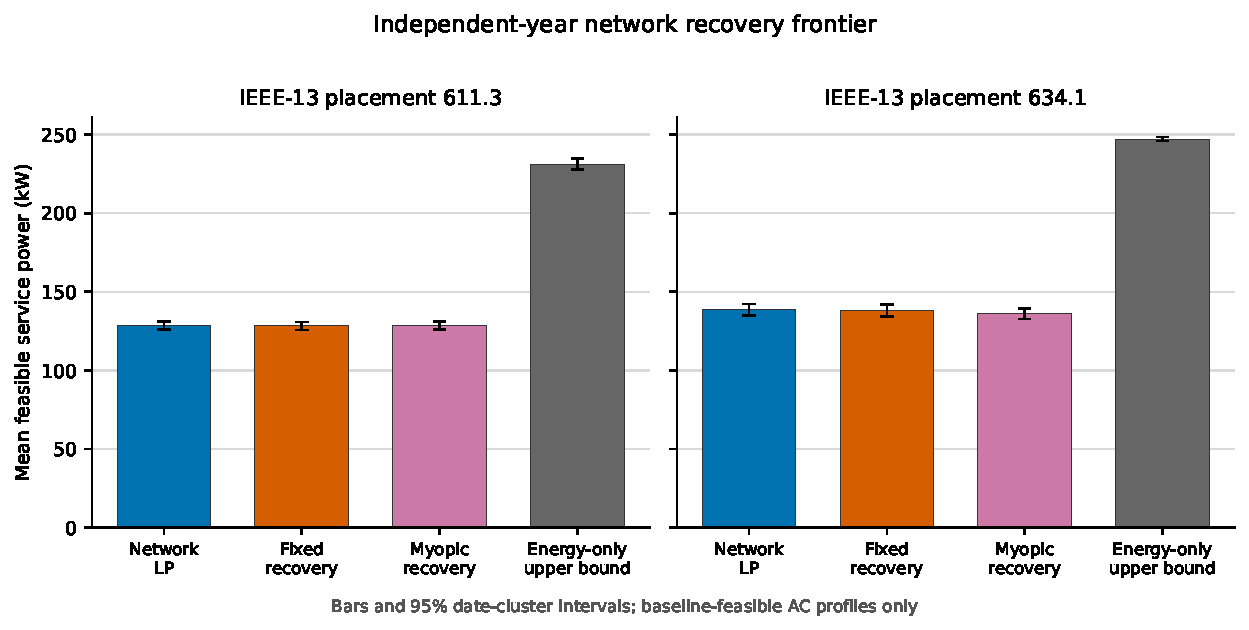
\includegraphics[width=0.99\linewidth]{fig1_external_frontier}
\caption{Mean feasible service power and descriptive 95\% date-cluster intervals. The energy-only bars are copper-plate counterfactuals; their schedules fail AC replay and are not deliverable offers.}
\label{fig:frontier}
\end{figure}

\subsection{AC replay and failure audit}
The full-horizon and fixed-recovery schedules replayed successfully on all 2,188 baseline-feasible units at both placements. The myopic schedule also replayed successfully at 611.3 and on 2,187 of 2,188 units at 634.1; the single failed replay was a boundary event with voltage and transformer loading readbacks only marginally above the declared limits. The energy-only schedule failed on all 2,188 baseline-feasible units at both placements. Its upper-bound service power is therefore a diagnostic of network optimism, not a feasible contract.

\begin{figure}[t]
\centering
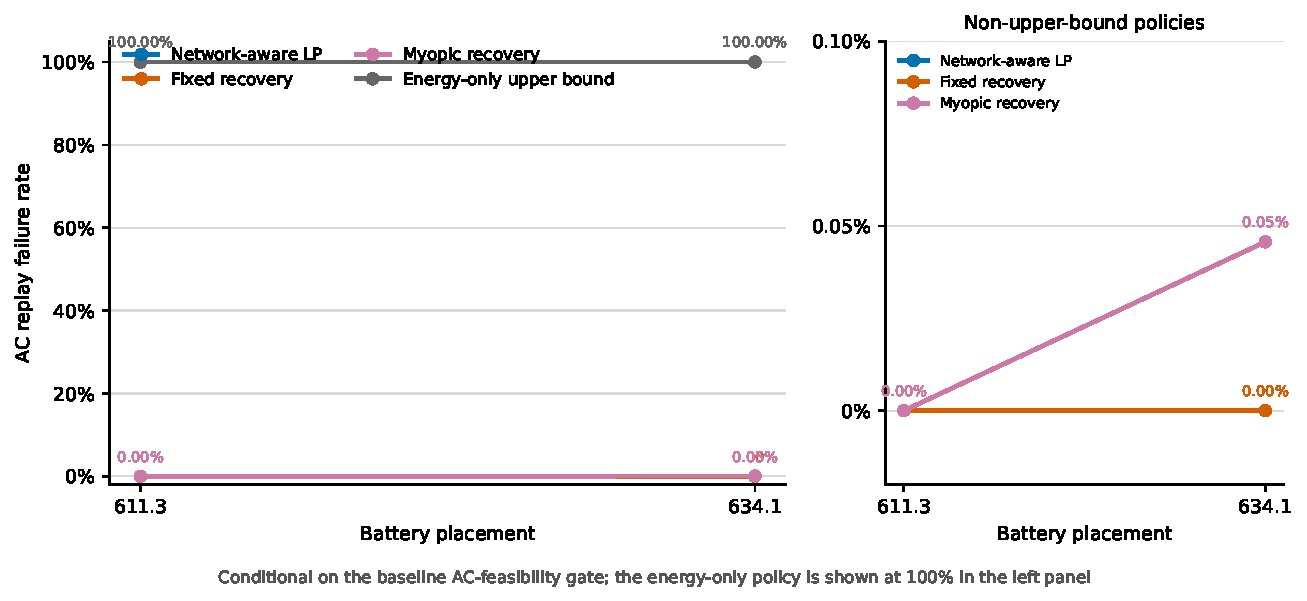
\includegraphics[width=0.99\linewidth]{fig3_failure_rates}
\caption{Conditional AC replay failure rates. The left panel retains the 100\% energy-only counterfactual failure rate; the right panel resolves the much smaller rates of the other policies.}
\label{fig:failure}
\end{figure}

\subsection{Recovery trajectory and headroom mechanism}
The representative trace shows that service calls and recovery windows occur at different AC charge limits. The full-horizon benchmark moves charging within the allowed recovery windows to satisfy the second call and the terminal SOC, whereas fixed recovery follows the same ratio regardless of the time-varying limit. At 634.1, the observed LP--myopic difference is positively associated with the recovery-window charge-headroom range (Spearman $\rho=0.440$; Pearson $r=0.508$ over 2,188 paired units). At 611.3, the LP--myopic difference is identically zero, so its correlation is undefined. These correlations are descriptive and do not establish a causal effect of placement.

\begin{figure}[t]
\centering
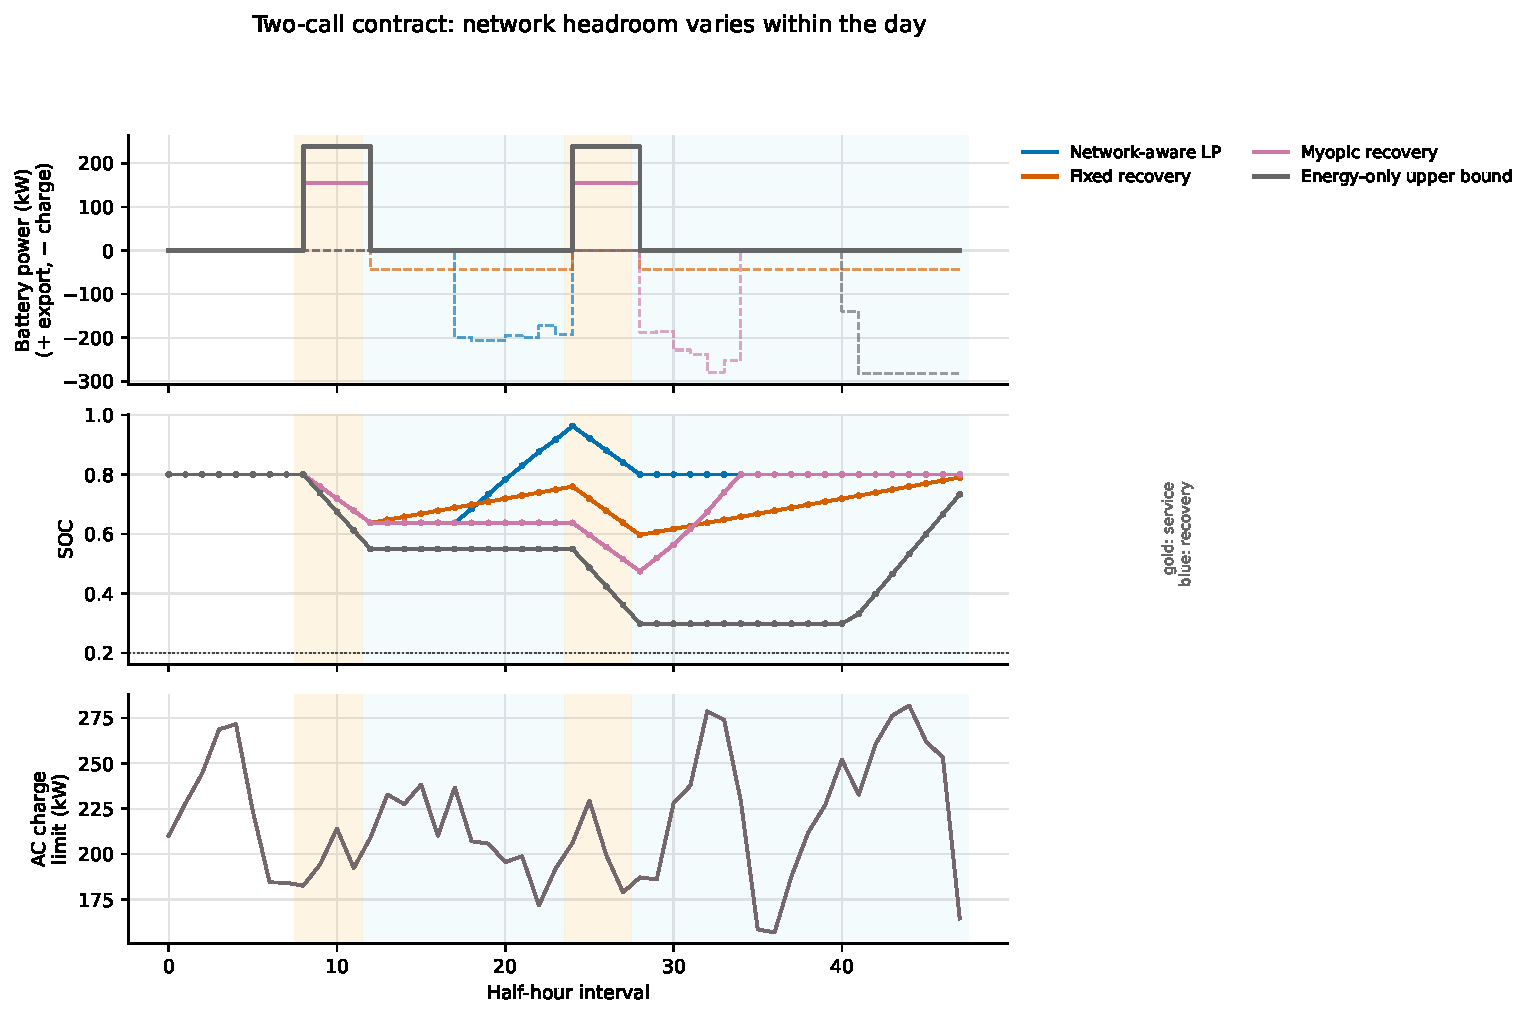
\includegraphics[width=0.99\linewidth]{fig2_recovery_trace}
\caption{Representative 48-interval trace. Gold shading marks the two service windows and blue shading marks the recovery windows. Solid curves show export; dashed curves show charging as negative battery power.}
\label{fig:trace}
\end{figure}

\begin{figure}[t]
\centering
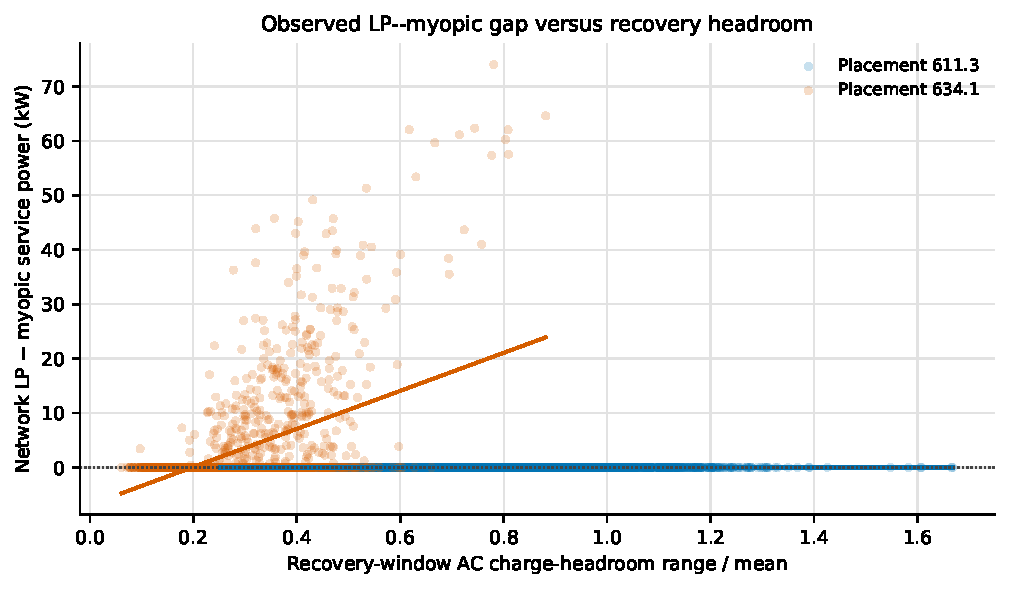
\includegraphics[width=0.82\linewidth]{fig4_headroom_mechanism}
\caption{Observed LP--myopic service-power difference against the recovery-window AC charge-headroom range divided by its mean. Lines are descriptive fits; the plot is not a causal test.}
\label{fig:mechanism}
\end{figure}

\section{Discussion}
The benchmark produces two operational findings. First, replacing time-varying feeder limits with an energy-only bound can overstate the service offer by roughly \kw{103}--\kw{109} at the tested placements, and that counterfactual fails AC replay for every baseline-feasible unit. Second, the value of anticipatory recovery depends on the electrical placement. At 611.3 the myopic rule is already sufficient for the frozen contract, while at 634.1 the full-horizon schedule gains about \kw{2.4} on average. A DSO can therefore use this workflow as an offline screening step: evaluate the proposed repeated service at the candidate location, inspect the recovery headroom, and retain the full-horizon result as a model-based benchmark before adding forecasts or online control.

The result is narrower than a chance-constrained procurement policy. The full-horizon benchmark sees the realized future and does not price flexibility, model forecast error, or optimize a market-clearing objective. The bootstrap intervals describe variation in the retained profile sample; they are not delivery guarantees for unobserved events. The small placement-dependent effect also shows why a generic claim that network-aware recovery always improves an offer would be unsupported by this experiment.

\section{Limitations}
The quantitative study uses one public IEEE 13-node feeder and two single-phase placements. The IEEE 123-node model is retained only as an adapter diagnostic because its baseline gate fails under the same limits. The battery is an active-power surrogate with fixed efficiencies and $Q=0$; inverter apparent-power limits, reactive power, degradation, temperature, protection actions, and field telemetry are not represented. Snapshot AC bounds and replay establish model-based feasibility, not physical delivery. The public profiles and fixed stress embedding do not cover all feeders, climates, customer populations, or market rules. Finally, the external dates are non-contiguous after a strict completeness mask, and the hindsight benchmark overstates what an online controller could know.

\section{Conclusions}
We developed an AC--SOC benchmark for repeated distribution-flexibility services. On a strict external-date evaluation, the full-horizon recovery schedule delivered \kw{128.526} at placement 611.3 and \kw{138.511} at 634.1 by the date-cluster estimand. Its value relative to a myopic rule was zero at 611.3 and \kw{2.433} at 634.1, while the energy-only counterfactual failed AC replay for all baseline-feasible units. The findings support a practical screening rule: a repeated offer should be checked against the recovery headroom at its electrical location, and an energy-only envelope should not be treated as deliverable service. Extending this benchmark to forecast-aware control, reactive-power inverters, additional feeders, and an explicit economic objective is required before a market recommendation can be made.

\section*{CRediT authorship contribution statement}
\textbf{Siqiang Zhao:} Conceptualization, Methodology, Software, Validation, Formal analysis, Investigation, Data curation, Visualization, Writing -- original draft. \textbf{Fengxiang Zhang:} Supervision, Writing -- review \& editing. The author order and contribution statement were confirmed by both authors.

\section*{Funding}
No dedicated external funding was received for this work.

\section*{Declaration of competing interest}
The authors declare that they have no known competing financial interests or personal relationships that could have appeared to influence the work reported in this paper.

\section*{Acknowledgements}
No additional acknowledgements are requested.

\section*{Data and code availability}
The public profile source, preprocessing metadata, source hashes, frozen group mapping, derived external-date manifest, experiment outputs, figures, and tests are provided in the development repository at \url{https://github.com/Zhaosiqiang/RecoveryFlex-AE}. The exact archival release tag and persistent DOI will be inserted after the manuscript and code package are frozen. No private participant-level data are claimed.

\section*{Declaration of generative AI and AI-assisted technologies in the writing process}
OpenAI Codex/ChatGPT and Manus were used as editorial and programming assistants for code organization, figure-generation support, drafting, and internal consistency checks. The authors reviewed and verified all scientific claims, methods, data handling, figures, and final text and remain fully responsible for the content. No AI tool is an author and no confidential or restricted data were provided to an AI tool.

\begin{thebibliography}{11}
\bibitem{Evans2022Recovery} M. P. Evans, S. H. Tindemans, D. Angeli, Flexibility framework with recovery guarantees for aggregated energy storage devices, IEEE Trans. Smart Grid 13 (2022) 3519--3531. doi:10.1109/TSG.2022.3173900.
\bibitem{Giraldo2023RiskEV} J. S. Giraldo, N. B. Arias, P. P. Vergara, M. Vlasiou, G. Hoogsteen, J. L. Hurink, Estimating risk-aware flexibility areas for electric vehicle charging pools via AC stochastic optimal power flow, J. Mod. Power Syst. Clean Energy 11 (2023) 1247--1256. doi:10.35833/MPCE.2022.000452.
\bibitem{Xiao2025SRC} J. Xiao, C. Li, G. He, Z. Lv, G. Sun, Y. Zhou, H. Liang, Flexible resource security regulating capability for distribution systems: Concept, method, and applications, Applied Energy 382 (2025) 125253. doi:10.1016/j.apenergy.2024.125253.
\bibitem{Lankeshwara2025DOE} G. Lankeshwara, R. Sharma, M. R. Alam, R. Yan, T. K. Saha, Development and validation of a dynamic operating envelopes-enabled demand response scheme in low-voltage distribution networks, Applied Energy 382 (2025) 125150. doi:10.1016/j.apenergy.2024.125150.
\bibitem{Cheng2026FOR} T. Cheng, J. Dai, D. Qiu, Z. Han, H. Sheng, H. Zhong, G. Strbac, Q. Xia, C. Kang, Coordinated optimal dispatch of storage-like resources based on dynamic feasible operation region aggregation, Applied Energy 424 (2026) 128444. doi:10.1016/j.apenergy.2026.128444.
\bibitem{Wanapinit2022FlexBidding} N. Wanapinit, J. Thomsen, A. Weidlich, Integrating flexibility provision into operation planning: A generic framework to assess potentials and bid prices of end-users, Energy 261 (2022) 125261. doi:10.1016/j.energy.2022.125261.
\bibitem{Wang2026Communication} S. Wang, Z. Wu, M. Zhou, Communication-dependent flexibility planning in digitalized distribution systems via dynamic storage reservation, Applied Energy 426 (2026) 128736. doi:10.1016/j.apenergy.2026.128736.
\bibitem{Ausgrid2011} Ausgrid, Solar home electricity data, public data archive, 2011. https://data.gov.au/data/dataset/5ab48b70-5e99-47d3-9193-5c34a2676d93 (accessed 3 October 2026).
\bibitem{OpenDSS13} Electric Power Research Institute, IEEE 13-node test feeder, OpenDSS distribution system examples, 2009. https://sourceforge.net/projects/electricdss/.
\end{thebibliography}
\end{document}
